%%%% Small single column format, used for CIE, CSUR, DTRAP, JACM, JDIQ, JEA, JERIC, JETC, PACMCGIT, TAAS, TACCESS, TACO, TALG, TALLIP (formerly TALIP), TCPS, TDSCI, TEAC, TECS, THRI, TIIS, TIOT, TISSEC, TIST, TKDD, TMIS, TOCE, TOCHI, TOCL, TOCS, TOCT, TODAES, TODS, TOIS, TOIT, TOMACS, TOMM (formerly TOMCCAP), TOMPECS, TOMS, TOPC, TOPLAS, TOPS, TOS, TOSEM, TOSN, TRETS, TSAS, TSC, TSLP, TWEB.
% \documentclass[format=acmsmall, review=false, screen=true]{acmart}

%%%% Large single column format, used for IMWUT, JOCCH, PACMPL, POMACS, TAP, PACMHCI
\documentclass[acmlarge]{acmart}
%%%% Large double column format, used for TOG
% \documentclass[acmtog, authorversion]{acmart}

%%%% Generic manuscript mode
%\documentclass[manuscript, review, screen]{acmart}
%\setcitestyle{super,sort&compress}
%\citestyle{acmnumeric}
\usepackage{booktabs} % For formal tables
%\usepackage{hyperref}

%\usepackage[ruled]{algorithm2e} % For algorithms
%\usepackage{listings}
%\usepackage{glossaries} % For abbreviations
%\usepackage[acronym,nonumberlist]{glossaries-extra}

%\loadglsentries{acronym_list}


% Load basic packages
%\usepackage{balance}       % to better equalize the last page
%\usepackage{graphics}      % for EPS, load graphicx instead
%\usepackage[T1]{fontenc}   % for umlauts and other diaeresis
%\usepackage{txfonts}
%\usepackage{mathptmx}
%\usepackage[pdflang={en-US},pdftex]{hyperref}
%%\usepackage{color}
%%\usepackage{booktabs}
%%\usepackage{textcomp}
%%\usepackage{gensymb}



% Package for algorithmic code
\usepackage{algorithm}
\usepackage[noend]{algpseudocode}
\usepackage{subcaption}
\makeatletter
\def\BState{\State\hskip-\ALG@thistlm}
\makeatother


% Metadata Information
%\acmJournal{IMWUT}
%\acmVolume{0}
%\acmNumber{0}
%\acmArticle{0}
%\acmYear{2018}
%\acmMonth{3}

%\acmBadgeL[http://ctuning.org/ae/ppopp2016.html]{ae-logo}
%\acmBadgeR[http://ctuning.org/ae/ppopp2016.html]{ae-logo}

% Copyright
%\setcopyright{acmcopyright}
%\setcopyright{acmlicensed}
%\setcopyright{rightsretained}
\setcopyright{usgovmixed}
%\setcopyright{cagov}
%\setcopyright{cagovmixed}

% DOI
%\acmDOI{0000001.0000001}


% Document starts
\begin{document}


% Title portion
\title{Investigating Affective Responses toward In-Video Pedestrian Crossing Actions using Camera and Physiological Sensors}

\author{Shruti Rao \textsuperscript{1},
    Surjya Ghosh \textsuperscript{1},
    Gerard Pons \textsuperscript{1},
    Thomas R\"{o}ggla \textsuperscript{1},
    Abdallah El Ali \textsuperscript{1},
    Pablo Cesar \textsuperscript{1, 2}}
\affiliation{
  \institution{\textsuperscript{1} Distributed \& Interactive Systems, Centrum Wiskunde \& Informatica}
  \institution{\textsuperscript{2} Delft University of Technology}
  \country{The Netherlands}}
\email{contact s.rao@cwi.nl}

\renewcommand\shortauthors{Rao et al.}

\keywords{empathic car, pedestrian non-verbal behaviour, driver emotion recognition, physiological sensing, thermal sensing}

\maketitle

\section*{Abstract}
\textbf{Motivation:} 
Inferring driver affective states during non-verbal driver-pedestrian interactions is significant for developing empathic, in-car interfaces \cite{koch2021drivers}. This is because emotions that arise during driving scenarios are known to adversely impact driving behaviour \cite{2015:tf:jeon, sucha2017pedestrian, locken2019should}. In this exploratory work, we investigated the impact of non-verbal, pedestrian crossing actions from the \textit{Joint Attention for Autonomous Driving (JAAD)} \cite{2017:IV:rasouli} dataset on participants’  affective responses (emotion self-reports, physiological responses and facial temperatures). 
\\
% Specifically, we ask: \textit{How do people's affective responses vary in response to different non-verbal, pedestrian crossing actions shown through video stimuli?}


\noindent \textbf{User Study:}  
We conducted an in-lab study where participants with driving experience (\textit{N=21}) watched $10$ non-verbal, pedestrian crossing videos from the \textit{JAAD} dataset \cite{2017:IV:rasouli, Ghosh2022}. We recorded participants' real-time, 9-point emotion (valence and arousal) self-reports \cite{bradley1994measuring}, heart rate, pupil diameter, skin conductance, and facial temperature responses for each video (experimental setup in Figure \ref{fig:exp_setup}).
\\

\noindent \textbf{Results:} 
We find that positive, non-verbal pedestrian crossing actions in the videos elicit higher valence (pleasantness) ratings from participants, while non-positive (excitement) actions elicit higher arousal. Different pedestrian crossing actions in the videos also have a significant ($p<0.05$) influence on participants' heart rate, pupil diameter, skin conductance, and facial temperatures. As a result, our work offers two key contributions - (1) Validation of non-verbal, pedestrian crossing stimuli (JAAD videos) that influence participants' affective states though multi-modal physiological and camera sensors. (2) Empirical findings which reveal that non-verbal, pedestrian actions influence participants' self-reported emotions (valence and arousal), physiological signals and facial temperatures. Our findings provide a first step toward enabling in-car empathic interfaces that draw on behavioural and physiological sensing to in-situ infer driver emotions during non-verbal pedestrian interactions.

\begin{figure}[!htbp]
    \centering	
        \begin{subfigure}[t]{0.32\textwidth}
        \centering        
        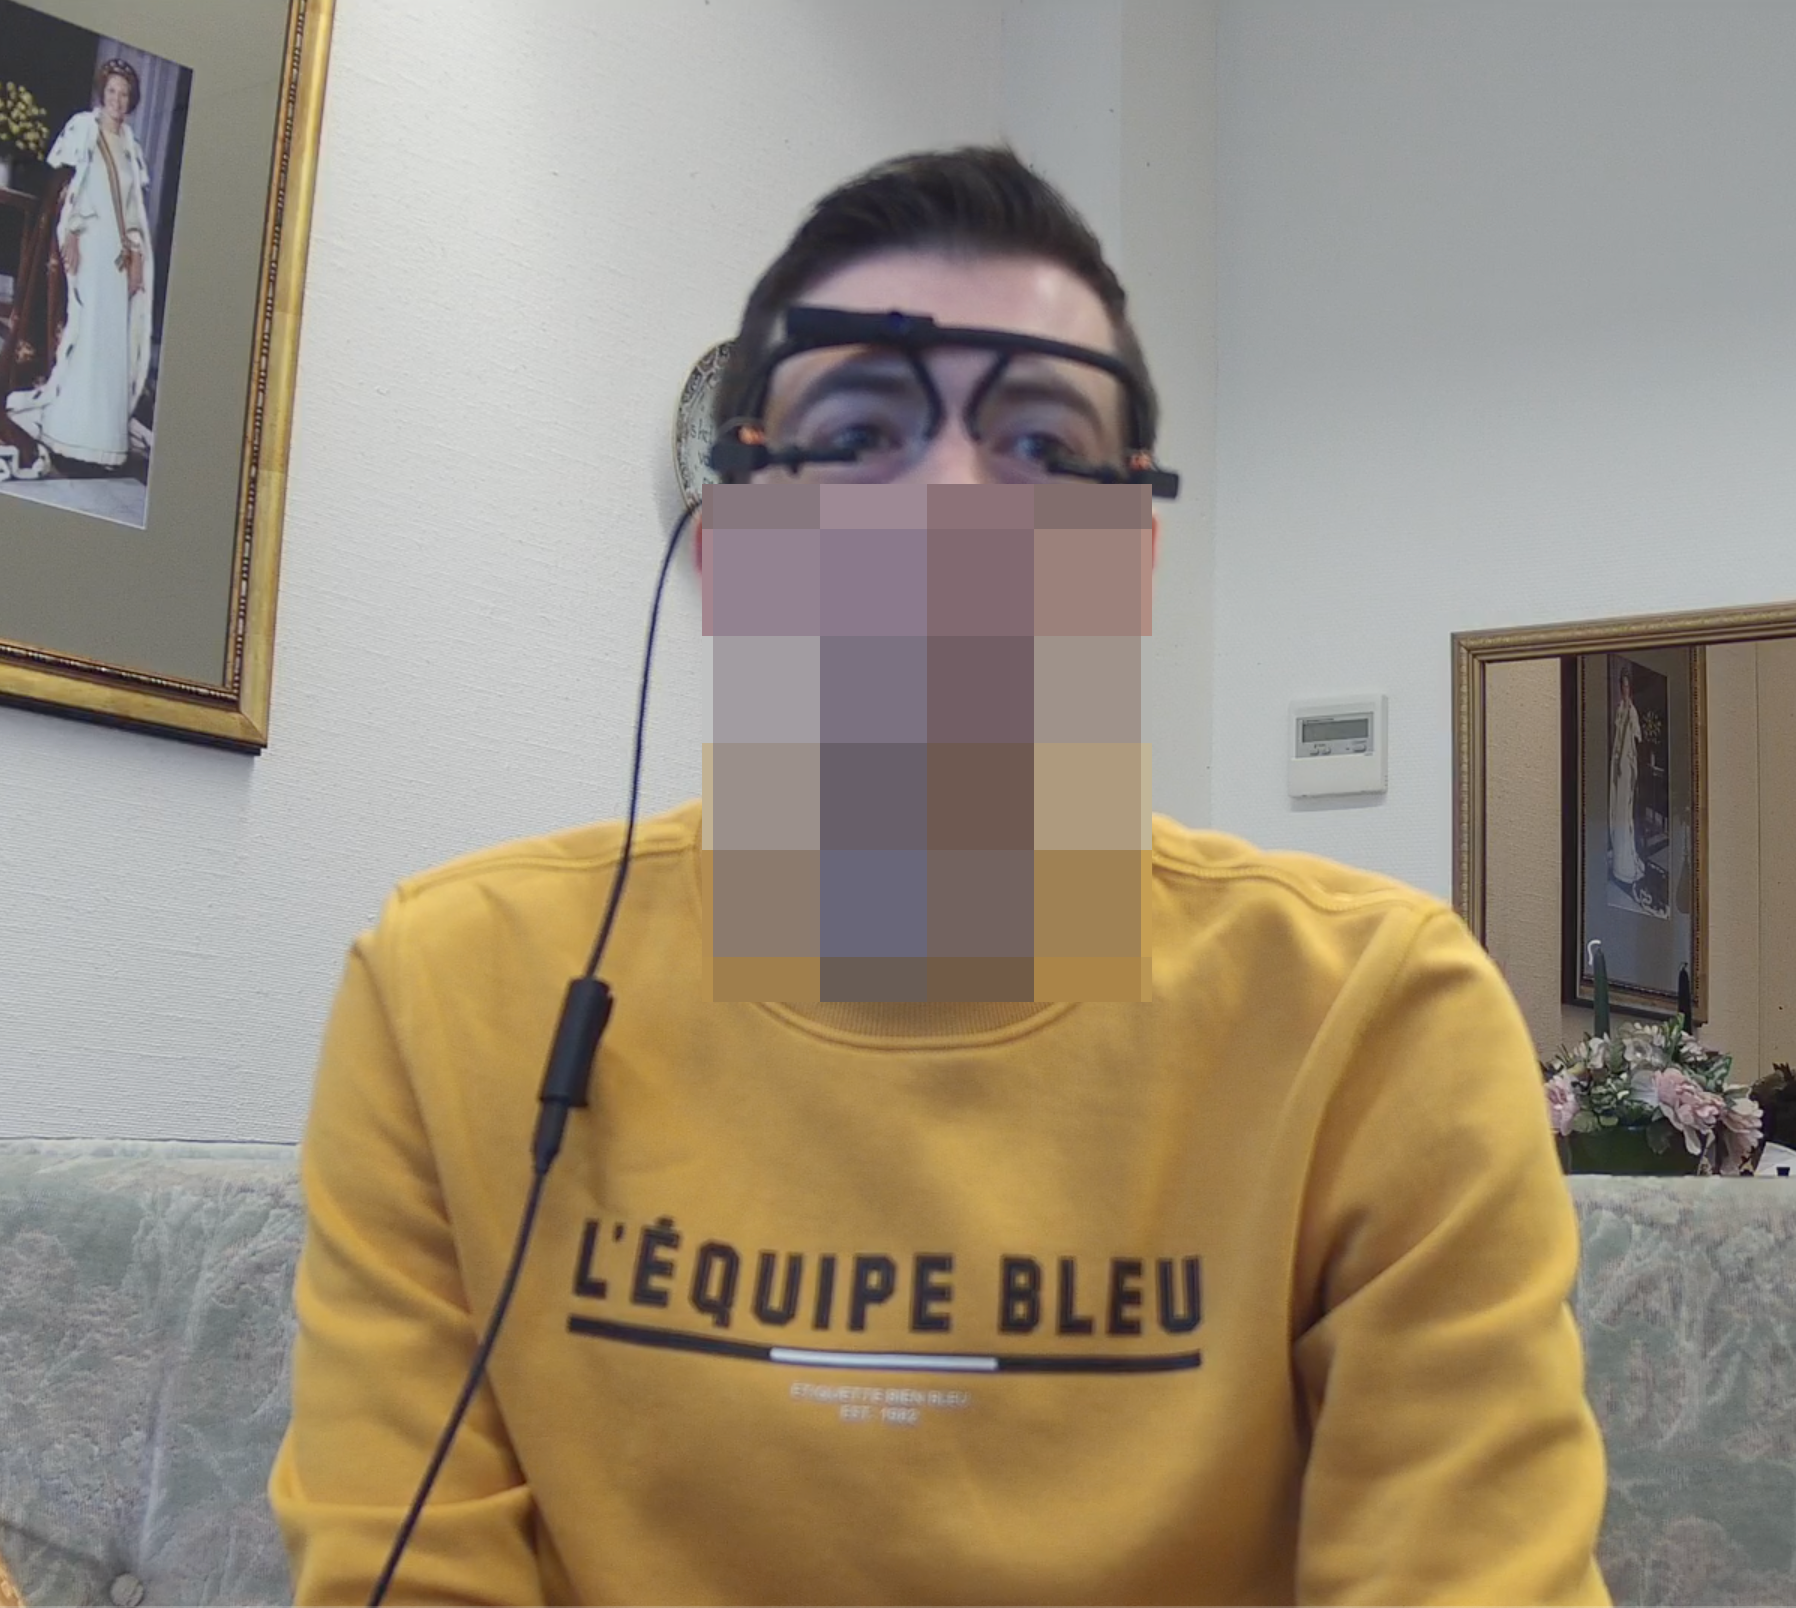
\includegraphics[width=\linewidth]{./images/anon_participant.png}
        \caption{Participant wearing the Pupil Labs eye tracker while watching video stimuli.}
        \label{fig:particpant_wearing_eye_tracker}
        \end{subfigure}%
        ~
        \begin{subfigure}[t]{0.27\textwidth}
        \centering        
        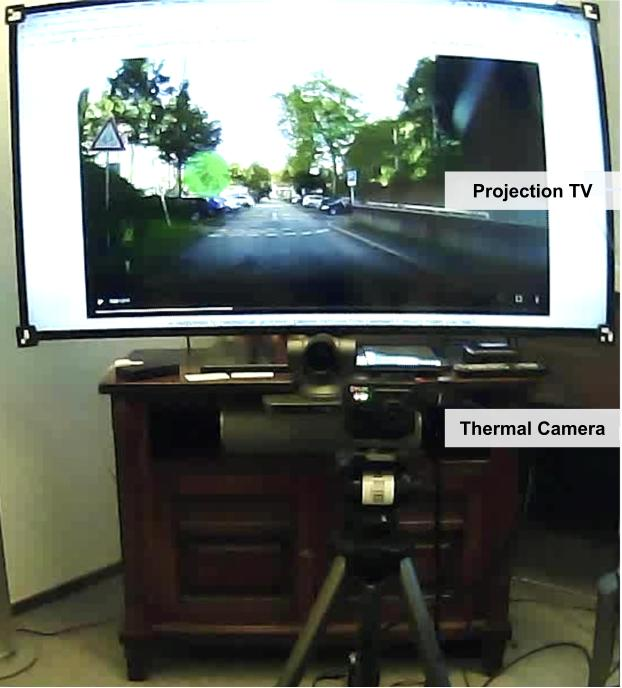
\includegraphics[width=\linewidth]{./images//val_study_setup.jpg}
        \caption{Thermal Camera and projection screen placement.}
        \label{fig:projector_setup}
        \end{subfigure}
        ~
        \begin{subfigure}[t]{0.40\textwidth}
        \centering        
        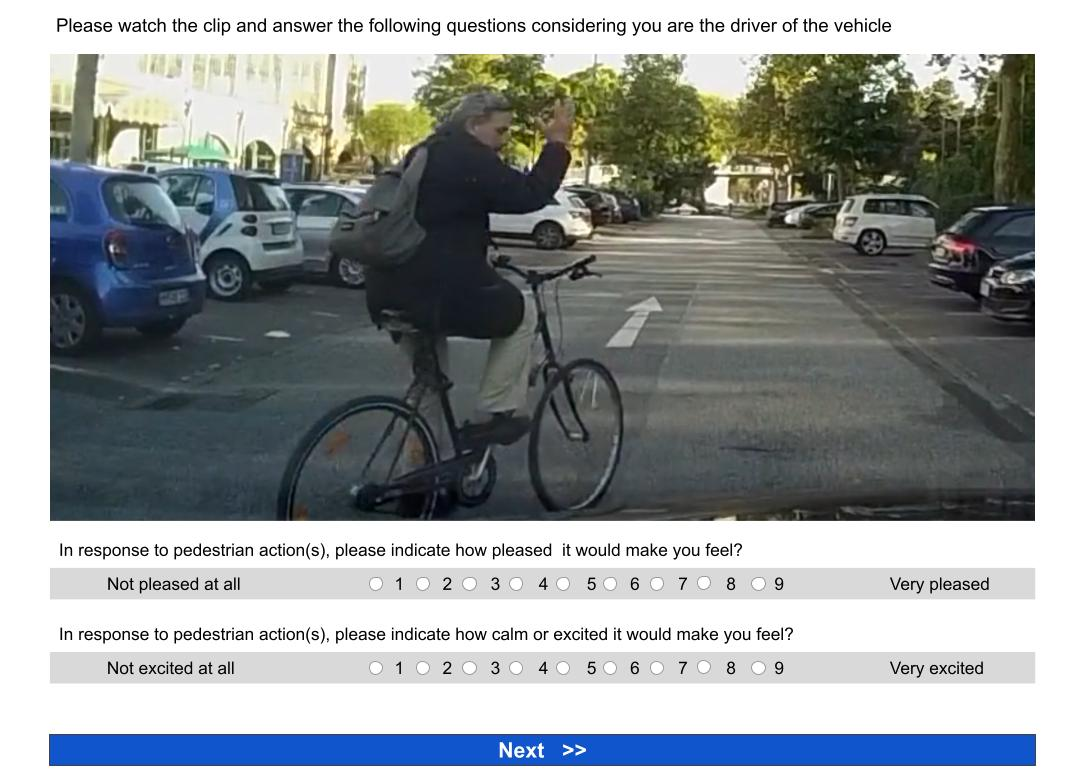
\includegraphics[width=\linewidth]{./images/video_page.jpg}
        \caption{The web-based user interface displays the video stimuli and records the participant's valence and arousal ratings after each video.}
        \label{fig:validation_study_video_page}
        \end{subfigure}
    \caption{Experiment setup with thermal camera and projection screen. Participants wear Pupil Labs eye tracker and watch the projection screen which shows the web-based user interface for viewing and rating driver-affect inducing stimuli.}
    \label{fig:exp_setup}
\end{figure}



% While our study lacks ecological validity (being an in-lab controlled setup), and does not address the robustness of detected participant signals towards just-in-time interventions, our results may be used for the development of emotion recognition models. These models can leverage driver affective cues (physiological, behavioural and thermal) during driver-pedestrian interactions as part of an emotion self-regulation framework for improving road safety. 





\bibliographystyle{ACM-Reference-Format}
\bibliography{report}
\end{document}
